%
% fdm.tex
%
% (c) 2020 Prof Dr Andreas Müller, Hochschule Rapperswil
%
\section{Finite Differenzen
\label{section:finite-differenzen}}
\rhead{Finite Differenzen}
Jedes Lösungsverfahren für partielle Differentialgleichungen muss die
unendlich vielen Freiheitsgrade, die eine Funktion
$u\colon\Omega\to\mathbb R$ enthalten kann, auf eine endlich Zahl von
Variablen reduzieren, für die sich ein Gleichungssystem aufstellen 
lässt, welches dann mit einer der früher studierten Methoden
gelöst werden kann.

%
% Gitter und Ableitungen
%
\subsection{Gitter und Ableitungen
\label{pde:subsection:gitter}}
Eine einfache Methode, die Funktion $u$ eine endliche Menge von Parametern
zu reduzieren, ist, nur die Werte in einzelnen Punkten des Gebietes 
$\Omega$ zu verwenden.
Als Beispiel betrachten wir ein Gebiet $\Omega\subset\mathbb R^2$
in der Ebene.
Dazu betrachten wir die Punkte
\[
x_{ik} = (ih_x, kh_y) \in \mathbb R^2
\qquad
i,k\in\mathbb Z,
\]
sie bilden ein Gitter $\Gamma$ mit Gitterkonstante oder Schrittweite
$h_x$ in $x$-Richtung und $h_y$ in $y$-Richtung.

Die Funktion $u(x,y)$ nimmt in den Punkten $x_{ik}$ die Werte
$u_{ik} = u(x_{ik})$ an.
Eine approximative Lösung der Differentialgleichung ist also
die Bestimmung der Werte $u_{ik}$ für die Punkte $x_{ik}$, die in
$\Omega$ liegen, für die also $x_{ik}\in\Omega$ gilt.
Dazu müssen jetzt die Randbedingungen und die Differentialgleichung
übersetzt werden in Gleichungen für die Unbekannten $u_{ik}$.

\subsubsection{Dirichlet-Randbedingungen}
Dirichlet-Randbedingungen geben die Werte auf dem Rand vor.
Liegt ein Punkt $x_{ik}$ des Gitters $\Gamma$ auf dem Rand $\partial\Omega$
von $\Omega$, dann geben die Dirichlet-Randbedingungen den Wert
dieser Variablen vor.
Es ist daher anzustreben, das Gitter $\Gamma$ so zu wählen, dass 
der Rand durch Gitterpunkte verläuft.
Ein gekrümmter Rand wird daher im Allgmeinen durch eine Kurve durch
die Gitterpunkte approximiert werden müssen.

\subsubsection{Erste Ableitungen}
\begin{figure}
\centering
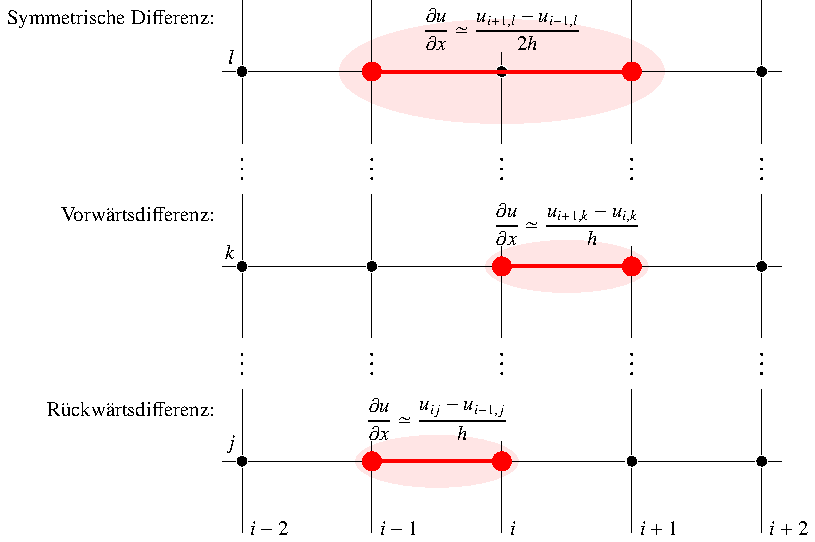
\includegraphics{chapters/70-pde/images/derivatives.pdf}
\caption{Approximation der ersten Ableitung mit verschiedenen
Differenzausdrücken
\label{buch:pde:1abldiff}}
\end{figure}
Die naheliegenste Approximation für die Differentialgleichung besteht
darin, die Ableitungen durch Differenzenquotienten zu ersetzen (siehe 
Abbildung~\ref{buch:pde:1abldiff}).
Mit der oben eingeführten Notation können die ersten Ableitungen durch
die sogenannten {\em Vorwärtsdifferenzen}
\index{Vorwärtsdifferenz}%
\begin{align}
\frac{\partial u}{\partial x} (x_{ik}) 
&\simeq
\frac{u(x_{i+1,k}) - u(x_{ik})}{h_x}
&
&\text{und}
&
\frac{\partial u}{\partial y} (x_{ik}) 
&\simeq
\frac{u(x_{i,k+1}) - u(x_{ik})}{h_y}
\label{chapter:pde:approx1st}
\end{align}
approximiert werden (Abbildung~\ref{buch:pde:1abldiff} Mitte).
Die Genauigkeit der Approximation kann offenbar verbessert werden, 
indem $h_x$ und $h_y$ verkleinert werden.

Der Fehler der Approximation~\eqref{chapter:pde:approx1st} ergibt sich
aus dem Mittelwertsatz der Differentialrechnung.
Es gibt Zahlen $\xi$ und $\eta$ zwischen $ih_x$ und $(i+1)h_x$
bzw.~$kh_y$ und $(k+1)h_y$ derart, dass
\begin{align*}
\frac{u(x_{i+1,k}) - u(x_{ik})}{h_x}
&=
\frac{\partial u}{\partial x}(\xi, kh_y)
&
&\text{und}
&
\frac{u(x_{i,k+1}) - u(x_{ik})}{h_y}
&=
\frac{\partial u}{\partial x}(ih_x, \eta).
\end{align*}
Dies zeigt, dass die Approximation~\eqref{chapter:pde:approx1st}
nicht für die Werte der Ableitungen im Punkt $x_{ik}$ repräsentativ 
sein kann.
Alternativ könnten statt der Vorwärtsdifferenzen die {\em Rückwärtsdifferenzen}
\index{Rückwärtsdifferenze}
\begin{align}
\frac{\partial u}{\partial x} (x_{ik}) 
&\simeq
\frac{u(x_{ik}) - u(x_{i-1,k})}{h_x}
&
&\text{und}
&
\frac{\partial u}{\partial y} (x_{ik}) 
&\simeq
\frac{u(x_{ik}) - u(x_{i,k-1})}{h_y}
\label{chapter:pde:approxrueckwaerts}
\end{align}
verwendet werden (Abbildung~\ref{buch:pde:1abldiff} unten).
Die Genauigkeit wird dadurch jedoch nicht verbessert, die Punkte
$(\xi,kh_y)$ und $(ih_x,\eta)$, an dem diese Ableitungswerte angenommen
werden, liegen jetzt einfach links bzw.~unterhalb von von $x_{ik}$.

Die Vorwärtsdifferenzen~\eqref{chapter:pde:approx1st} sind also
fehlerhaft genauso wie
die Rückwärtsdifferenzen~\eqref{chapter:pde:approxrueckwaerts},
wenngleich in eine andere Richtung.
Ein Mittelweg könnte ein Differenzenquotient
\begin{align*}
\frac{\partial u}{\partial x}(x_{ik})
&=
\frac{u_{i+1,k}-u_{i-1,k}}{2h_x}
&&\text{und}
&
\frac{\partial u}{\partial y}(x_{ik})
&=
\frac{u_{i,k+1}-u_{i,k-1}}{2h_y}
\end{align*}
über ein symmetrisches Interval der doppelten Länge.
\index{symmetrische Differenz}%
Diese sogenannten {\em symmetrische Differenzen}
(Abbildung~\ref{buch:pde:1abldiff}) sind eher repräsentativ
für die Steigung im Punkt $x_{ik}$, dafür ist die Genauigkeit wegen des
doppelt so langen Intervals kleiner.

\begin{beispiel}
\begin{figure}
\centering
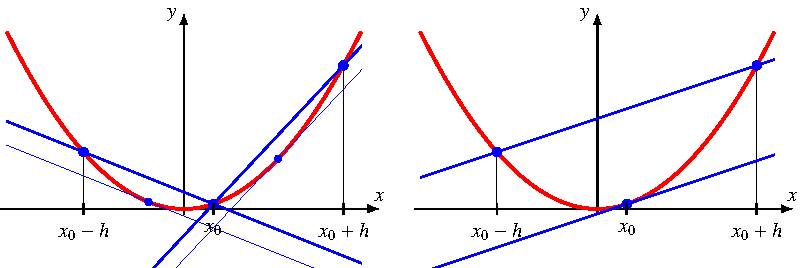
\includegraphics{chapters/70-pde/images/diffex.pdf}
\caption{Differenzenquotienten für die Funktion $f(x)=x^2$.
Die Vorwärts- und Rückwärtsdifferenzen im Punkt $x_0$ ergeben Approximationen
für die Ableitungen, die mit der wahren Ableitung im Punkt $x_0\pm \frac{h}2$
übereinstimmen.
Die symmetrische Differenz im Punkt $x_0$ ergibt genau die Steigung von $f(x)$
im Punkt $x_0$.
\label{buch:pde:diffex}}
\end{figure}
Um die Unterschiede zwischen den Fehlern der verschiedenen
Differenzapproximationen besser zu verstehen, approximieren wir die
Ableitungen der Funktion $f(x)=x^2$ im Punkt $x_0$ und bestimmen den
Fehler sowie den Punkt, in dem die Approximation den korrekten Ableitungswert
annimmt.
Die Vorwärts-, Rückwärts- und symmetrischen Differenzen sind
\begin{align*}
f'(x_0)
&\simeq
\frac{f(x_0+h)-f(x_0)}{h}
=
\frac{(x_0+h)^2-x_0^2}{h}
=
2x_0+h
&&=
f'(x_0 + {\textstyle\frac12}h)
\\
&\simeq
\frac{f(x_0)-f(x_0-h)}{h}
=
\frac{x_0+^2-(x_0-h)^2}{h}
=
2x_0-h
&&=
f'(x_0 - {\textstyle\frac12}h)
\\
&\simeq
\frac{f(x_0+h)-f(x_0-h)}{2h}
=
\frac{(x_0+h)^2-(x_0-h)^2}{2h}
=
\frac{4x_0h}{2h}=2x_0
&&=
f'(x_0).
\end{align*}
Für eine quadratische Funktion liefert also die symmetrische Differenz
den exakten Wert der Ableitung im Punkt $x_0$, während die Vorwärts-
und Rückwertsdifferenzen die Ableitungen in Punkten zwischen
den Gitterpunkten rechts bzw.~links von $x_0$
(Abbildung~\ref{buch:pde:diffex}).
\end{beispiel}

\subsubsection{Zweite Ableitungen}
\begin{figure}
\centering
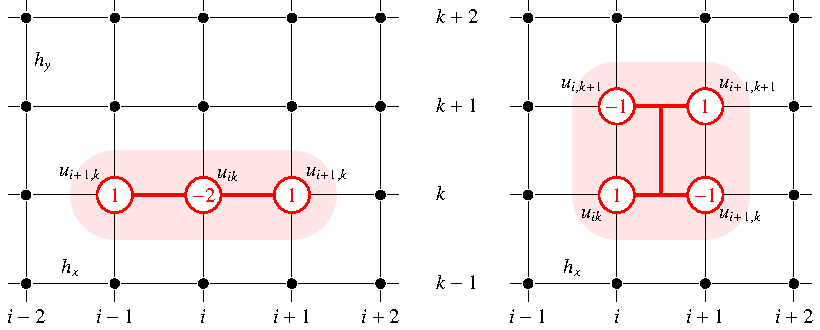
\includegraphics{chapters/70-pde/images/diff2.pdf}
\caption{Differenzenquotienten für die zweiten Ableitungen.
Links die zweite Ableitungen nach $x$, rechts die gemischte Ableitung.
In den roten Kreisen das Gewicht des zugehörigen Wertes der Funktion
im Differenzenquotienten.
\label{buch:pde:diff2}}
\end{figure}
Eine Approximation für die zweite Ableitung können wir erhalten als
Differenzenquotient aus der Vorwärts- und der Rückwärtsdifferenz:
\begin{align*}
\frac{\partial^2 u}{\partial x^2}(x_{ik})
&\simeq
\frac{1}{h_x}\biggl(
\frac{\partial u}{\partial x}(x_{i-\frac12,k})
-
\frac{\partial u}{\partial x}(x_{i+\frac12,k})
\biggr)
=
\frac{1}{h_x}
\cdot
\biggl(
\frac{u_{i+1,k}-u_{ik}}{h_x}
-
\frac{u_{ik}-u_{i-1,k}}{h_x}
\biggr)
\\
&=
\frac{u_{i+1,k}-2u_{ik}+u_{i-1,k}}{h_x^2}.
\end{align*}
Das Problem wird aber schwieriger, wenn eine gemischte Ableitung
approximiert werden soll.
Hier kann jede beliebige Kombination von Vorwärts- und Rückwärts-Differenzen
verwendet werden.
Mit Vorwärtsdifferenzen erhält man zum Beispiel
\begin{align*}
\frac{\partial^2u}{\partial x\,\partial y}(x_{ik})
&\simeq
\frac{1}{h_x}\biggl(
\frac{\partial u}{\partial y}(x_{i+1,k})
-
\frac{\partial u}{\partial y}(x_{ik})
\biggr)
\\
&=
\frac{1}{h_x}\biggl(
\frac{u_{i+1,k+1}-u_{i+1,k}}{h_y}
-
\frac{u_{i,k+1}-u_{ik}}{h_y}
\biggr)
\\
&=
\frac{1}{h_xh_y}(
u_{i+1,k+1}-u_{i+1,k}
-
u_{i,k+1}+u_{ik}
)
\end{align*}
Die in Abbildung~\ref{buch:pde:diff2} dargestellten ``Schablonen''
zeigen schematisch, wie die Ableitungen berechnet werden.
In den roten Kreisen um die beteiligten Knotenvariablen stehen die
Gewichte, mit denen die Knotenvariablen multipliziert werden müssen.

\subsubsection{Neumann-Randbedingungen}
Neumann-Randbedingungen geben die Ableitungen in Richtung der Normalen
auf dem Rand vor.
Die Diskretisation auf ein Gitter führt dazu, dass der Rand aus geraden
Teilstücken besteht, wo eine Normalenrichtung leicht zu definieren ist,
und Teilstücken, wo zusätzlicher Aufwand getrieben werden muss, überhaupt
die Richtung der Normalen zu definieren.
Für gerade Teilstücke des Randes können für die Approximation der
Normalableitung Vorwärts- oder Rückwärtsdifferenzen verwendet
werden.

\begin{beispiel}
Zur Illustration des Vorgehens approximieren wir die Normalableitungen
für das Rechteckgebiet mit Rändern $x=0$, $x=Nh_x$, $y=0$ und $y=Mh_y$,
welches in Abbildung~\ref{XXX} dargestellt ist.
In Punkten $x_{0k}$ und $x_{Nk}$ auf den vertikalen Rändern
oder in Punkten $x_{i0}$ und $x_{iM}$ auf den horizontalen Rändern
können wir Vorwärts- bzw.~Rückwärtsdifferenzen verwenden:
\begin{align*}
\frac{\partial u}{\partial n}(x_{0k})
=
\frac{\partial u}{\partial x}(x_{0k})
&\simeq
\frac{u_{1k}-u_{0k}}{h_x}
&&\text{und}&
\frac{\partial u}{\partial n}(x_{Nk})
=
\frac{\partial u}{\partial x}(x_{Nk})
&\simeq
\frac{u_{Nk}-u_{N-1,k}}{h_x},
\\
\frac{\partial u}{\partial n}(x_{i0})
=
\frac{\partial u}{\partial y}(x_{i0})
&\simeq
\frac{u_{i1}-u_{i0}}{h_y}
&&\text{und}&
\frac{\partial u}{\partial n}(x_{iM})
=
\frac{\partial u}{\partial y}(x_{iM})
&\simeq
\frac{u_{iM}-u_{i,M-1}}{h_y}.
\end{align*}
Natürlich gelten die oben formulierten Vorbehalte bezüglich der
Zuverlässigkeit dieser Approximation, wir haben aber nicht die Möglichkeit,
symmetrische Differenzen zu verwenden, da keine Funktionswerte ausserhalb
des Gebietes bekannt sind.
\end{beispiel}

TODO: XXX Abbildung, die die Probleme mit Neumann-Randbedingungen im
Gitter illustriert

\subsubsection{Das Poisson-Problem}
\begin{figure}
\centering
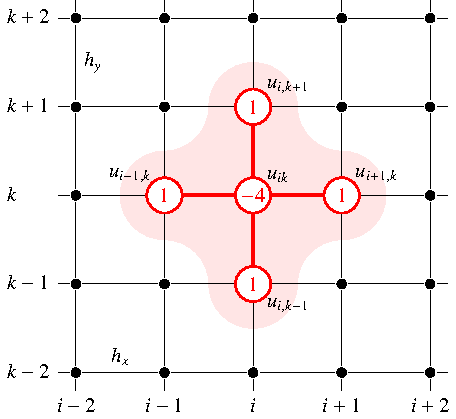
\includegraphics{chapters/70-pde/images/laplace.pdf}
\caption{Approximation des Laplace-Operators mit Summen von symmetrischen
Differenzen.
In den roten Kreisen die Gewichte, mit denen die Knotenvariablen 
multipliziert werden müssen, um den Ausdruck
\eqref{pde:eqn:poissongl} zu ergeben.
\label{buch:pde:laplace}}
\end{figure}
Das Poisson-Problem ist die Differentialgleichung
\begin{equation}
\frac{\partial^2 u}{\partial x^2}
+
\frac{\partial^2 u}{\partial y^2}
=
f
\label{buch:pde:poissondgl}
\end{equation}
auf einem Gebiet $\Omega$, wobei wir als Beispiel ein Quadrat
$\Omega = (0,1) \times (0,1)$ wählen.
Die abstrakte Theorie sagt, dass die Lösung der Differentialgleichung
eindeutig bestimmt ist, Randwerte $u(x)=g(x)$ für $x\in\partial\Omega$
vorgegeben werden.

\begin{figure}
\centering
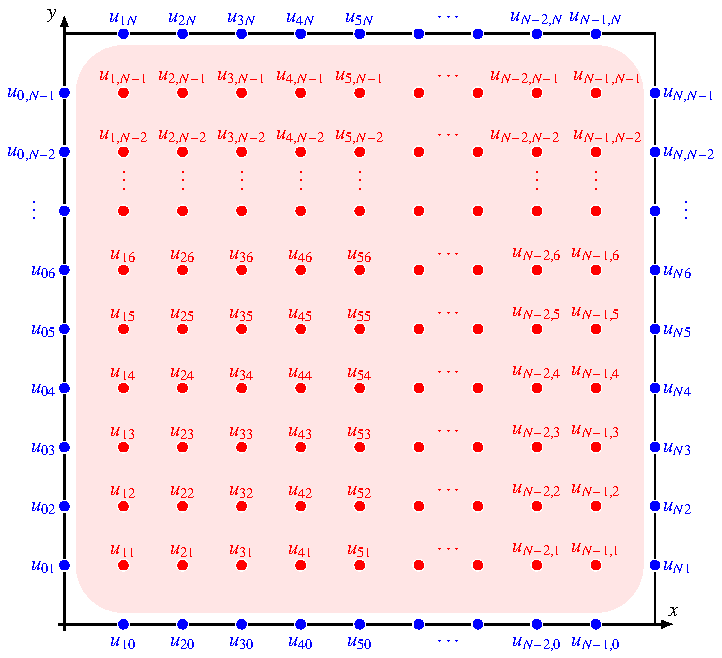
\includegraphics{chapters/70-pde/images/poisson.pdf}
\caption{Diskretisiertes Gebiet für die Differentialgleichung.
Die Werte in den blauen Punkten auf dem Rand sind durch die Randbedingungen
gegeben, nur die Werte in den roten Punkten müssen bestimmt werden.
\eqref{buch:pde:poissondgl}.
\label{buch:pde:poissongebiet}}
\end{figure}
Wir diskretisieren das Gebiet (Abbildung~\ref{buch:pde::poissongebiet})
mit Hilfe des Gitters mit Gitterkonstanten
$h=h_x=h_y=1/N$.
Wir erhalten die $(N+1)^2$ Unbekannten $u_{ik}$ mit $0\le i\le N$ und 
$0\le k\le N$.
Die Randbedingungen legen die Werte
\begin{align*}
u_{0k}&= g(0, kh)
&
u_{Nk}&= g(1, kh)
&&0\le k\le N
\\
u_{i0}&=g(ih,0)
&
u_{iN}&=g(ih,N)
&&
1\le i\le N
\end{align*}
fest.
$4N$ Unbekannte sind also bereits bestimmt, es bleiben noch
$(N+1)^2-4N = N^2-2N+1=(N-1)^2$ innere Werte zubestimmen.

Die Differentialgleichung kann für jeden Punkt im Inneren des Gebietes
$\Omega$ aufgestellt werden, es gilt
\begin{align}
\frac{\partial^2 u}{\partial x^2}(u_{ik})
+
\frac{\partial^2 u}{\partial y^2}(u_{ik})
&=
\frac{u_{i+1,k}-2u_{ik}+u_{i-1,k}}{h^2}
+
\frac{u_{i,k+1}-2u_{ik}+u_{i,k-1}}{h^2}
\notag
\\
f_{ik}=f(x_{ik})
&=
\frac{1}{h^2} ( u_{i+1,k} + u_{i-1,k} + u_{i,k+1} + u_{i,k-1} - 4u_{ik}).
\label{pde:eqn:poissongl}
\end{align}
Alle diese $(N-1)^2$ Gleichungen sind linear.
Insbesondere haben wir gleich viele Gleichungen wie Unbekannte und 
dürfen daher davon ausgehen, dass, wie sich auch beweisen lässt, das
lineare Gleichungssystem
\eqref{pde:eqn:poissongl} 
für die verbleibenden Unbekannten regulär ist.
Die Diskretisation führt also die Lösung der partiellen Differentialgleichung
auf die Lösung eines linearen Gleichungssystems zurück.


%
% Explizite und implizite Verfahren
%
\subsection{Explizite und Implizite Verfahren
\label{pde:subsection:explizitimplizit}}
Der vorangegangene Abschnitt hat gezeigt, dass für die Approximation
der Differentialgleichung und der Randbedingungen verschiedene 
Optionen zur Verfügung stehen.
In diesem Abschnitt soll am Beispiel der Wärmeleitungsgleichung
illustriert werden, wie daraus verschiedene Näherungsverfahren für
die Lösung werden, die ganz unterschiedliche Konvergenzeigenschaften
haben können.

\subsubsection{Die Wärmeleitungsgleichung}
TODO: XXX Graphik mit Definitionsbereich und Diskretisation für die
Wärmeleitungsgleichung.

Als Beispiel für die bisher entwickelte Theorie versuchen wir,
auf dem Gebiet
\[
\Omega = \{ (x,t)\;|\; 0 < x < 1\wedge 0<t\}
\]
die  Wärmeleitungsgleichung
\[
\frac{\partial u}{\partial t}
=
\kappa\frac{\partial^2 u}{\partial x^2}
\]
lösen mit den Randbedingungen
\[
\begin{aligned}
u(x,0)&=f(x)&&x\in[0,1]
\\
\frac{\partial u}{\partial n}(x,t)=\frac{\partial u}{\partial x}(x,t)&=0&&x\in \{0,1\}.
\end{aligned}
\]
Die Funktion $u(x,t)$ beschreibt die Temperatur an der Position $x$
eines Stabes der Länge $1$ zur Zeit $t$, der zur Zeit $t=0$ die 
Temperaturverteilung $f(x)$ hatte und an den Enden isoliert ist.

Zur Diskretisation verwenden wir ein Gitter mit Gitterkonstanten
$h_x=1/N$ und $h_t$.
Die zu bestimmenden Unbekannten sind die $u_{ik}$ mit
$0\le i\le N$ und $k\ge 0$.
Die Randbedingungen auf dem Rand $t=0$ geben die Werte 
\[
u_{i0} = u(ih_x,0) = f(ih_x)
\]
vor.
Die Neumann-Randbedingungen am linken und rechten Rand können mit Hilfe
der Vorwärts- bzw.~Rückwärts-Differenzen approximiert werden:
\begin{align*}
\frac{\partial u}{\partial n}(x_{0k})
&\simeq
\frac{u_{1k}-u_{0k}}{h_x}
=
0
&&\text{und}&
\frac{\partial u}{\partial n}(x_{0k})
&\simeq
\frac{u_{Nk}-u_{N-1,k}}{h_x}
=
0
\intertext{Dies bedeutet, dass die beiden Werte nahe des Randes
gleich sind}
u_{0k}&=u_{1k}&&\text{und}&u_{Nk}&=u_{N-1,k}.
\end{align*}
Die Differentialgleichung verwendet die zweite Ableitung nach $x$, 
für die wir die Approximation
\[
\frac{\partial^2u}{\partial x^2}(x_{ik})
=
\frac{u_{i+1,k}-2u_{ik}+u_{i-1,k}}{hx^2}
\]
verwenden können.
Für die erste Ableitung nach der Zeit könnten Vorwärts- oder
Rückwärts-Differenzen verwendet werden, in beiden Fällen entsteht
ein unvermeidbarer Fehler und ein jeweils anderes numerisches
Lösungsverfahren.

\subsubsection{Euler-Verfahren}

\subsubsection{Rückwärts}

\subsubsection{Implizites Verfahren}

%
% Stabilität und Computational Mode
%
\subsection{Stabilität und Computational Mode
\label{pde:subsection:stabilitaet}}






